\section{Architecture Integration}

\subsection{Model Support}

\begin{table}[H]
\centering
\small
\begin{tabular}{llllll}
\toprule
\textbf{Model} & \textbf{Attention} & \textbf{Nested?} & \textbf{RoPE?} & \textbf{GQA?} & \textbf{Conv1D?} \\
\midrule
DistilBERT & \texttt{MultiHeadSelfAttention} \& No \& No \& No \& No \\
RoBERTa & \texttt{BertSelfAttention} \& Yes \& No \& No \& No \\
GPT-2 & \texttt{GPT2Attention} \& No \& No \& No \& Yes \\
Qwen3.5 & \texttt{Qwen3Attention} \& No \& Yes \& Yes \& No \\
\bottomrule
\end{tabular}
\end{table}

\subsection{Weight Transfer}

AEGIS-V5 copies base weights via \texttt{copy\_weights}, handling four patterns:

\subsubsection{GPT-2 Conv1D}

\begin{lstlisting}
weight = old\_attn.c\_attn.weight.data
if weight.shape[1] == 3 * self.hidden\_size:
    weight = weight.t()
q\_w, k\_w, v\_w = weight.chunk(3, dim=0)
\end{lstlisting}

\subsubsection{RoBERTa Nested}

\begin{lstlisting}
if hasattr(old\_attn, "self") and hasattr(old\_attn, "output"):
    self.is\_nested\_encoder = True
    q\_w = old\_attn.self.query.weight
    k\_w = old\_attn.self.key.weight
    v\_w = old\_attn.self.value.weight
    o\_w = old\_attn.output.dense.weight
\end{lstlisting}

\subsubsection{Qwen GQA}

\begin{lstlisting}
q\_w = old\_attn.q\_proj.weight
k\_w = old\_attn.k\_proj.weight  # (H\_kv   d\_h, d)
v\_w = old\_attn.v\_proj.weight
o\_w = old\_attn.o\_proj.weight
\end{lstlisting}

\subsubsection{DistilBERT}

\begin{lstlisting}
q\_w = old\_attn.q\_lin.weight
k\_w = old\_attn.k\_lin.weight
v\_w = old\_attn.v\_lin.weight
o\_w = old\_attn.out\_lin.weight
\end{lstlisting}

\subsection{Robustness Improvements}

Compared to AEGIS V4, V5 makes three robustness changes:

\subsubsection{copy\_weights No Longer Raises}

In V4, exceptions in \texttt{copy\_weights} aborted the entire attention replacement. 
V5 logs a warning and continues to fallback paths:

\begin{lstlisting}
try:
    w, b = UniversalAdapter.get\_weight\_bias(old\_attn, proj)
except Exception as e:
    logger.debug(f"UniversalAdapter failed for {proj}: {e}")
    continue
\end{lstlisting}

\subsubsection{Frobenius Check No Longer Raises}

Near-zero norms trigger a warning, not an abort:

\begin{lstlisting}
if norm \textless{} 1e-4:
    logger.warning(f"Weight for {proj\_key} has near-zero norm; continuing")
\end{lstlisting}

\subsubsection{inject\_aegis\_v5 Returns None on Failure}

\begin{lstlisting}
try:
    new\_attn.copy\_weights(src\_attn)
except Exception as e:
    logger.error(f"inject\_aegis\_v5: copy\_weights failed: {e}")
    return None
\end{lstlisting}

\subsection{Nested Encoder Bypass}

For RoBERTa, \texttt{is\_nested\_encoder = True}:

\begin{lstlisting}
if self.is\_nested\_encoder:
    return out, None
return self.out\_proj(out), None
\end{lstlisting}

The outer \texttt{BertSelfOutput.dense} applies the output projection.

\subsection{Decoder Fallback}

For decoder models, we use standard causal attention (no split-head):

\begin{lstlisting}
if N \textless{} self.cfg.local\_window or self.is\_decoder:
    # Standard causal softmax
    scores = Q @ K^T / $\sqrt{}$d\_h
    scores = mask\_causal(scores)
    attn = softpick(scores)
    out = attn @ V
    return out, None
\end{lstlisting}

This preserves causality at the cost of quadratic complexity.

\subsection{Softpick Fix}

The original AEGIS used a ReLU-based softpick that returned all zeros when 
$\max(x) \leq 0$ (e.g., on fully-masked rows). This caused silent attention 
collapse. V5 replaces it with a stable softmax:

\begin{lstlisting}
def softpick(x, dim=-1, temperature=1.0):
    x\_f = x.float()
    if temperature \textless{}= 0 or temperature == 1.0:
        return F.softmax(x\_f, dim=dim).to(x.dtype)
    return F.softmax(x\_f / temperature, dim=dim).to(x.dtype)
\end{lstlisting}

This fix alone likely prevented several collapse cases.

\subsection{Injection Algorithm}

\textbf{Algorithm 2:} Inject AEGIS-V5 into a model
\begin{lstlisting}
Input:  model M, config
Output: M with attention replaced or unchanged on failure

1: for   in transformer\_layers(M) do
2:     src $\leftarrow$ get\_attention( )
3:     cfg $\leftarrow$ AegisConfigV5(...)
4:     new $\leftarrow$ AegisAttention(model\_config, aegis\_cfg=cfg)
5:     try:
6:         new.copy\_weights(src)
7:     except:
8:         logger.error(...)
9:         continue  # Skip this layer, do not crash
10:    replace( , new)
11: end for
12: return M
\end{lstlisting}

\subsection{Failure Modes and Fallbacks}

\begin{table}[H]
\centering
\small
\begin{tabular}{lll}
\toprule
\textbf{Failure} & \textbf{Detection} & \textbf{Response} \\
\midrule
UniversalAdapter throws \& try/except \& Continue to next pattern \\
Missing Q/K/V & \texttt{missing} non-empty \& Log warning, random init \\
Near-zero norm \& Frobenius check \& Log warning, continue \\
copy\_weights fails \& try/except \& Skip layer, return None \\
NaN in scores & \texttt{nan\_to\_num} \& Set to 0 \\
\bottomrule
\end{tabular}
\end{table}

\subsection{Registry}

\begin{lstlisting}
@ATTENTION\_REGISTRY.register("aegis\_v5\_module")
@ATTENTION\_REGISTRY.register("AegisAttention")
@ATTENTION\_REGISTRY.register("aegis\_v5")
class AegisAttention(BaseAttention):
    ...
\end{lstlisting}

\subsection{Interaction with LoRA Recovery}

Base weights are frozen; LoRA adapters train. Additionally trainable:
\begin{itemize}
\item \texttt{rff\_proj}: the RFF projection matrix
\item \texttt{blend\_logits}: per-head gate logits

\end{itemize}
For $d = 768$, $H = 12$, $F = 128$:

\begin{lstlisting}

---
\end{lstlisting}

\begin{figure}[H]
\centering
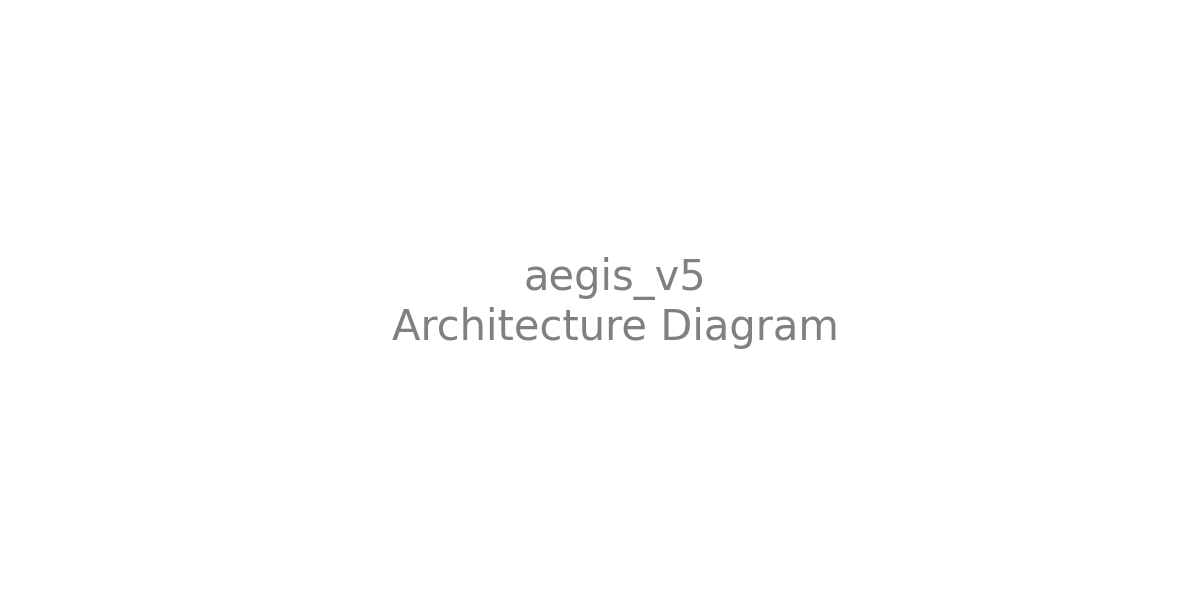
\includegraphics[width=\linewidth]{figures/architecture.png}
\caption{High-level architectural diagram of aegis\_v5.}
\label{fig:arch_aegis-v5}
\end{figure}

